%%%%%%%% ICML 2023 EXAMPLE LATEX SUBMISSION FILE %%%%%%%%%%%%%%%%%

\documentclass{article}

% Recommended, but optional, packages for figures and better typesetting:
\usepackage{microtype}
\usepackage{graphicx}
\usepackage{subfigure}
\usepackage{booktabs} % for professional tables
\usepackage{amsmath}
\usepackage{ifthen}
\usepackage{lipsum}
\usepackage{amsfonts}

\newcommand{\tz}[1]{{\color{magenta}TZ: #1}}
\newcommand{\jh}[1]{{\;\color{red}JH: #1}}
\newcommand{\bc}[1]{{\color{olive}BC: #1}}

% hyperref makes hyperlinks in the resulting PDF.
% If your build breaks (sometimes temporarily if a hyperlink spans a page)
% please comment out the following usepackage line and replace
% \usepackage{icml2023} with \usepackage[nohyperref]{icml2023} above.
\usepackage{hyperref}


% Attempt to make hyperref and algorithmic work together better:
\newcommand{\theHalgorithm}{\arabic{algorithm}}

% Use the following line for the initial blind version submitted for review:
\usepackage{icml2023}

% If accepted, instead use the following line for the camera-ready submission:
% \usepackage[accepted]{icml2023}

% For theorems and such
\usepackage{amsmath}
\usepackage{amssymb}
\usepackage{mathtools}
\usepackage{amsthm}

% if you use cleveref..
\usepackage[capitalize,noabbrev]{cleveref}

%%%%%%%%%%%%%%%%%%%%%%%%%%%%%%%%
% THEOREMS
%%%%%%%%%%%%%%%%%%%%%%%%%%%%%%%%
\theoremstyle{plain}
\newtheorem{theorem}{Theorem}[section]
\newtheorem{proposition}[theorem]{Proposition}
\newtheorem{lemma}[theorem]{Lemma}
\newtheorem{corollary}[theorem]{Corollary}
\theoremstyle{definition}
\newtheorem{definition}[theorem]{Definition}
\newtheorem{assumption}[theorem]{Assumption}
\theoremstyle{remark}
\newtheorem{remark}[theorem]{Remark}

% Todonotes is useful during development; simply uncomment the next line
%    and comment out the line below the next line to turn off comments
%\usepackage[disable,textsize=tiny]{todonotes}
\usepackage[textsize=tiny]{todonotes}


% The \icmltitle you define below is probably too long as a header.
% Therefore, a short form for the running title is supplied here:
\icmltitlerunning{Submission and Formatting Instructions for ICML 2023}


\newcommand{\norm}[1]{\left\lVert#1\right\rVert}
\DeclareMathOperator*{\argmin}{arg\,min}
\DeclareMathOperator*{\argmax}{arg\,max}
\newcommand{\transpose}{\mathsf{T}}

\newcommand*{\iidsim}{\overset{\text{i.i.d.}}{\sim}}


\begin{document}

\twocolumn[
% \icmltitle{The Anna Karenina Conjecture of Intelligence}
% \icmltitle{The Intelligence Bottleneck}
%\icmltitle{The Scaling Law of Representational Convergence}
\icmltitle{Cross Modal Representational Convergence: An Observation and a Theory}

% It is OKAY to include author information, even for blind
% submissions: the style file will automatically remove it for you
% unless you've provided the [accepted] option to the icml2023
% package.

% List of affiliations: The first argument should be a (short)
% identifier you will use later to specify author affiliations
% Academic affiliations should list Department, University, City, Region, Country
% Industry affiliations should list Company, City, Region, Country

% You can specify symbols, otherwise they are numbered in order.
% Ideally, you should not use this facility. Affiliations will be numbered
% in order of appearance and this is the preferred way.
\icmlsetsymbol{equal}{*}

\begin{icmlauthorlist}
\icmlauthor{Firstname1 Lastname1}{equal,yyy}
\icmlauthor{Firstname2 Lastname2}{equal,yyy,comp}
\icmlauthor{Firstname3 Lastname3}{comp}
\icmlauthor{Firstname4 Lastname4}{sch}
\icmlauthor{Firstname5 Lastname5}{yyy}
\icmlauthor{Firstname6 Lastname6}{sch,yyy,comp}
\icmlauthor{Firstname7 Lastname7}{comp}
%\icmlauthor{}{sch}
\icmlauthor{Firstname8 Lastname8}{sch}
\icmlauthor{Firstname8 Lastname8}{yyy,comp}
%\icmlauthor{}{sch}
%\icmlauthor{}{sch}
\end{icmlauthorlist}

\icmlaffiliation{yyy}{Department of XXX, University of YYY, Location, Country}
\icmlaffiliation{comp}{Company Name, Location, Country}
\icmlaffiliation{sch}{School of ZZZ, Institute of WWW, Location, Country}

\icmlcorrespondingauthor{Firstname1 Lastname1}{first1.last1@xxx.edu}
\icmlcorrespondingauthor{Firstname2 Lastname2}{first2.last2@www.uk}

% You may provide any keywords that you
% find helpful for describing your paper; these are used to populate
% the "keywords" metadata in the PDF but will not be shown in the document
\icmlkeywords{Machine Learning, ICML}

\vskip 0.3in
]

% this must go after the closing bracket ] following \twocolumn[ ...

% This command actually creates the footnote in the first column
% listing the affiliations and the copyright notice.
% The command takes one argument, which is text to display at the start of the footnote.
% The \icmlEqualContribution command is standard text for equal contribution.
% Remove it (just {}) if you do not need this facility.

%\printAffiliationsAndNotice{}  % leave blank if no need to mention equal contribution
\printAffiliationsAndNotice{\icmlEqualContribution} % otherwise use the standard text.

% \title{The Anna Karenina Conjecture of Intelligence}
% \date{April 2023}

\section{Introduction}

In multiple ways, the field of AI is converging. We can see this by comparing the years 2014 and 2024. In 2014, the dominant architecture for computer vision was the CNN while for NLP it was the RNN. Now both fields use transformers. In 2014 robots used handcrafted state representations, now robots are increasingly use reprsentations pretrained on vision or language tasks. What has led to this convergence? Is it a good thing? Will it continue? And where does it end?

This paper provides our perspectives on these questions. We target a specific kind of convergence: the convergence of representations of signals across modalities. We argue that 1) representations are converging, 2) this convergence opens up many new opportunities for taking advantage of it, and 3) representations are converging toward a probability distribution over physical state, which we will term $P(Z)$.

\begin{figure}[t]
    \centering
    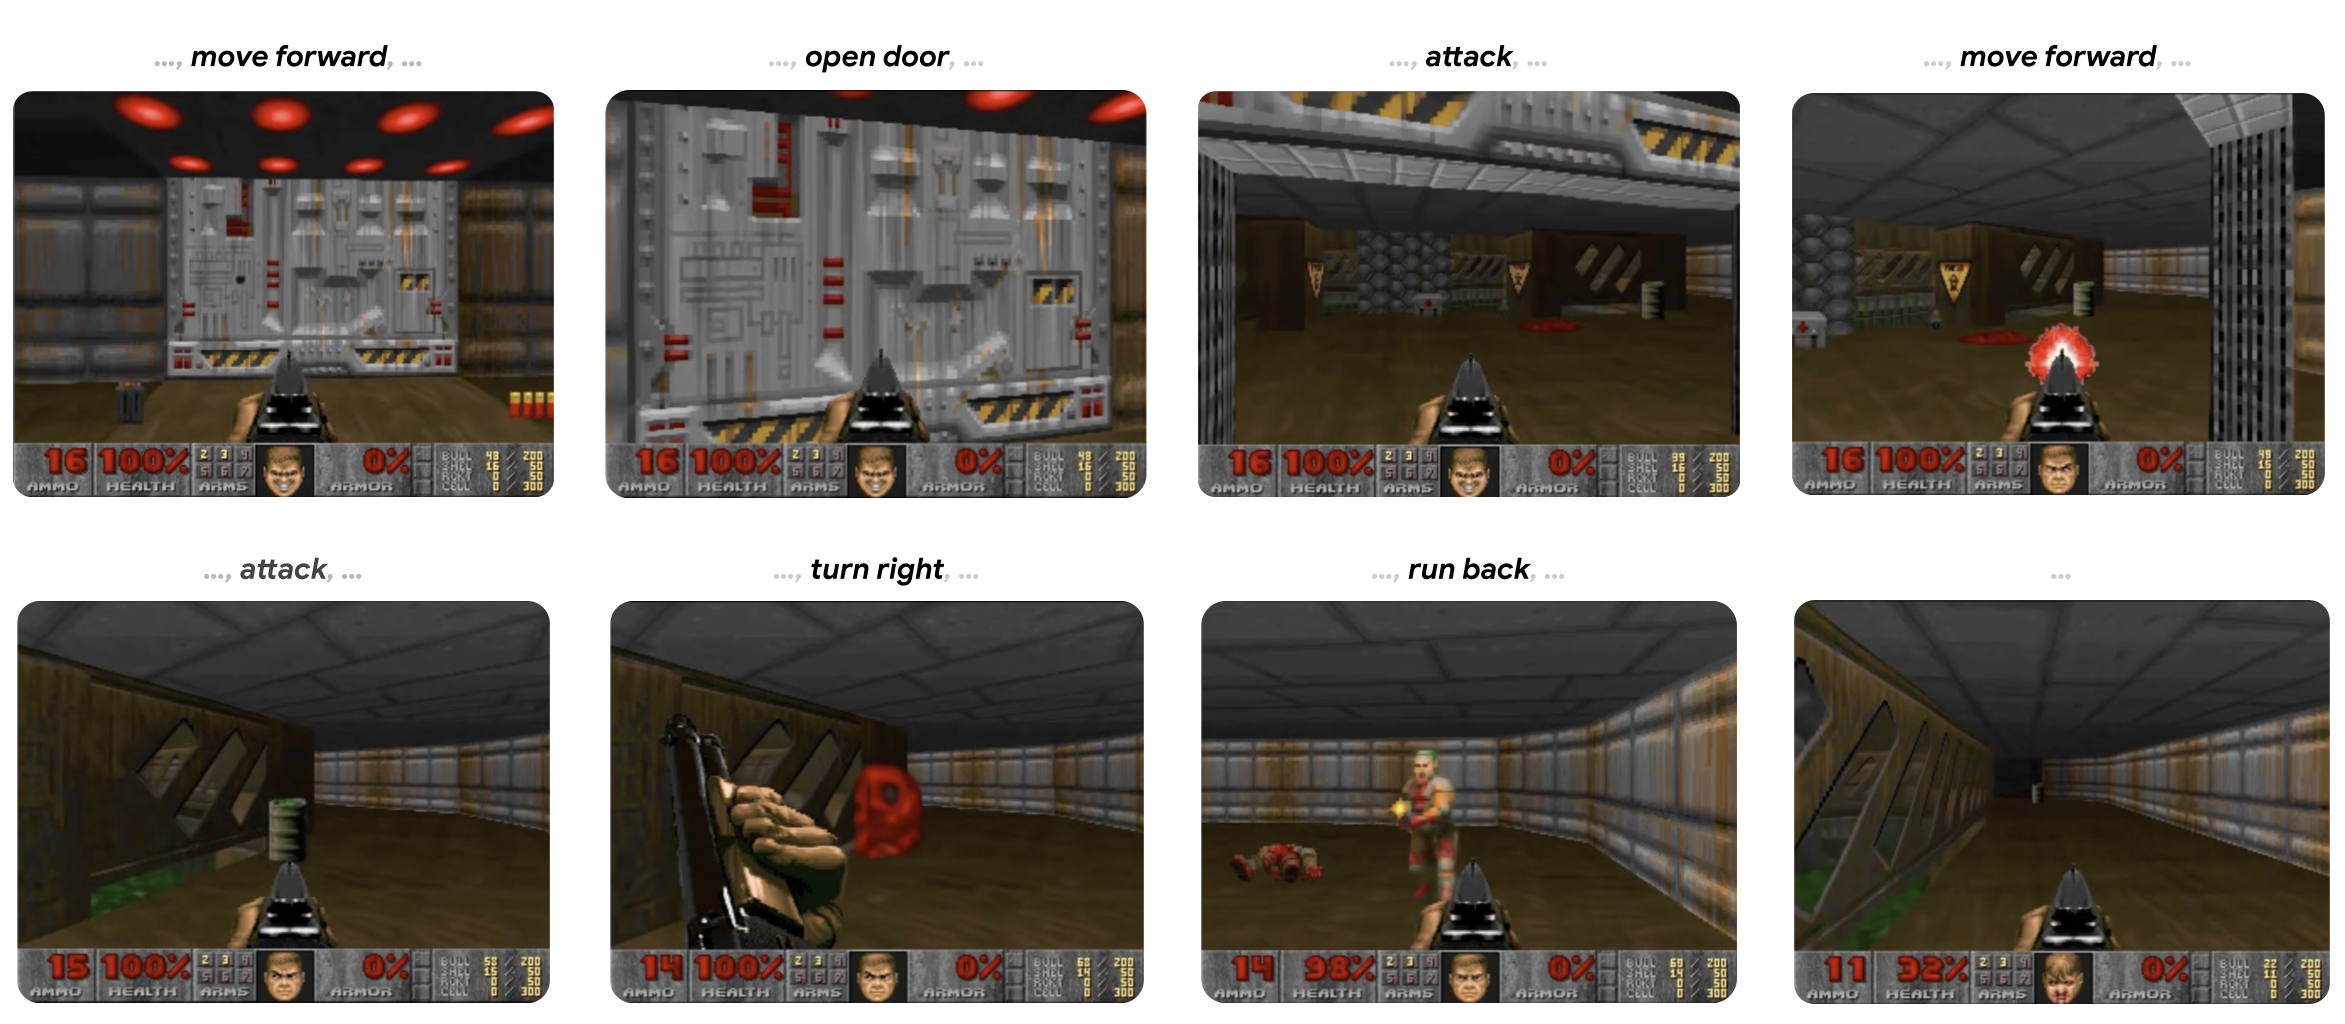
\includegraphics[width=1.0\linewidth]{figures/teaser.png}
    \caption{Representations are converging over time. Why? And what are they converging to?}
    \label{fig:convergence_over_time}
\end{figure}

\begin{abstract}
\lipsum[2]
\end{abstract}

\section{An Observation: Representational Alignment is Increasing over Time}

The motivation of this paper is that it \textit{feels like} AI representations are converging. We ran the following experiment to test if this feeling is valid.

We sampled a variety of models developed in different years, from 2012 to 2023. If models are converging, then the models in year $N$ should be more alike to one another than the models in year $M$ for $M<N$.

We measure how alike one model is to another using \texttt{CKA}. This metric assigns a high score to two models if they represent inputs in a similar way. In particular, $\texttt{CKA}(f_A,f_B)$ measures the similarity between the way model $f_A$ measures distance between inputs and the way model $f_B$ measures distance between the same inputs\footnote{Or matching inputs. If $f_A$ is an image encoder and $f_B$ is a text encoder, then \texttt{CKA} checks if $f_A$ measures distance between images in the same way as $f_B$ measures distance between the captions for those same images.}. Models $f_A$ and $f_B$ are both functions $\mathcal{X} \rightarrow \mathbb{R}^N$ that induce a distance metric $\norm{f_A(x_i) - f_A(x_j)}$. \texttt{CKA} is a standard method in the field of representational alignment \cite{XX}; we defer further discussion of it to the appendix.

Figure \ref{fig:convergence_over_time} shows our results. The average \texttt{CKA} between models is increasing over time. This is true for both vision models and for language models: in each subsequent year, two given vision models will tend to measure distance between images in more and more similar a way, and similarly for language models for distance between text. Remarkably, we also observe a cross modality convergence: the \texttt{CKA} between vision models and language models is also increasing over time.

Therefore, we conclude that our feeling is valid: over time, models, within and between modality, are measuring distance between items in more and more similar ways.

Next we turn our attention to explaining why this is happening.

\section{These trends can be explained by scale}

There are many reasons why we might see such a convergence: perhaps it's a social effect, where different communities talk more and all intellectual diversity collapses, or perhaps it is because we all use the same hardware, and the hardware determines properties of the representations \cite{hardware lottery}.

In this section, we point out a third possibility: models scale over time, and the larger the scale the greater the convergence.

To test this hypothesis, we run the following experiments. We define three kinds of scale: model parameter count, training data size, training flops. Functions of these attributes are commonly called scaling laws. Here we present a scaling law of representational alignment. For each scale variable, we create 10 evenly spaced bins. Then we plot \texttt{CKA} alignment within each bin. The results are shown in figures XX, YY, and ZZ.

Scale explains the trends to a similar degree as time did. Could it be that time is causal and scale simply correlates with time. If we look within a single year, holding time constant, we see the same effect of scale, as shown in figure XX. If we instead hold scale constant, the effect of time is much diminished. Therefore, we conclude that scale is a better explanation of the trends we are seeing.

\section{Why does scaling lead to convergence}

This is expected if the thing we are converging to is the solution to an optimization problem with a single global minimum\footnote{Or multiple minima that all induce the same distances~\cite{permutation invariance works}.}. Then if you optimize better (via scaling), of course you converge.


\section{If representations are converging, what are they converging to?}

In this section, we argue that representations are converging to $P(Z)$. We make a mathematical argument, then we show results on a toy world (colored shapes measured via images and text) and find that both vision and language indeed recover the same color similarity function (or shape similarity function), then we show that vit and llms also measure color-color distance in the same way.

One way to answer this question is to look at: what is the minimizer of common representation learning objectives? We will show that for several models they are some simple function of cooccurrences between events.


\subsection{We are converging toward the model that does well on everything, and there is only one such model}


\subsection{We are converging to a model of coocurrences}

Many theories of learning center on identifying associations between events that cooccur. First, we will show that both contrastive learning and predictive learning are optimized by simple functions of cooccurrence.

\subsubsection{Setup:} 
Assume that an observation of the world consists of a set of events, $\mathbf{A} = {A_0, \ldots, A_N}$. Each event is a discrete random variable that can take on values $a \in \mathcal{A}$. These events could denote, for example ``there is a dog in the scene'' or ``the sky is cloudy.'' (Capital letters are random variables and lowercase variables are realizations.)

The world generates data according to some distribution:
\begin{align}
    \mathbf{a} \sim P(\mathbf{A})
\end{align}

%For simplicity, we will assume that $N=2$ and $M_i = M \quad\forall\quad i$.

The methods we will consider below train an embedding $h: \mathcal{A} \rightarrow \mathbb{R}^d$. We will analyze the linear kernel $K$ over these embeddings:
\begin{align}
    K(a_i, a_j) \triangleq h(a_i)^\transpose h(a_j)
\end{align}

\subsubsection{Contrastive learning induces $K(a_i,a_j) = \texttt{PMI}(a_i,a_j)$}

Contrastive learning aligns positive pairs and pushes apart negative pairs. Define a positive pair as two cooccurring events and a negative pair as two random events from the marginals:\footnote{This definition describes common contrastive learners like SimCLR or SimCSE, in which the positive distribution is two patches/words that cooccur in the same image/paragraph. An observation of the world in those cases would be an image or a paragraph, and the events would be the patches in the image and the words in the paragraph.}
\begin{align}
    P^+(A_i,A_j) &\triangleq P(A_i,A_j), \quad A_i, A_j \in \mathbf{A}\\
    P^-(A_i,A_j) &\triangleq P(A_i)P(A_j)
\end{align}

Now we will analyze the InfoNCE objective:
\begin{align}
    \underset{\substack{
    a,a^+ \sim P^+ \\
    \{a^-_i\}_{i=1}^{M} \iidsim P^-
    }}{\mathbb{E}} \Bigg[\log \frac{f(a,a^+)}{f(a,a^+) + \sum_i f(a,a_i^-)} \Bigg]
\end{align}


The CPC paper proves that the optimal $f$ that minimizes this objective is $f(a_i,a_j) = \frac{1}{Z(a_j)}P(a_i | a_j)/P(a_i)$, where $Z(a_j) = \sum_{k=1}^M P(a_k | a_j)/P(a_k)$.

Now consider the following form for $f$, which is commonly used:
\begin{align}
    f(a_i,a_j) \triangleq e^{h(a_i)^\transpose h(a_j)}
\end{align}

Then we have the following kernel if the optimum is achieved:
\begin{align}
    f(a_i,a_j) &= e^{h(a_i)^\transpose h(a_j)}\\
    &= \frac{P(a_i | a_j)}{P(a_i)Z(a_j)}\\
    \log f(a_i,a_j) &= h(a_i)^\transpose h(a_j)\\
    &= \log \frac{P(a_i | a_j)}{P(a_i)} - \log Z(a_j)\\
    &= \texttt{PMI}(a_i,a_j) - \log Z(a_j)
\end{align}

But this optimum cannot be achieved since $f$ is symmetric and the rhs is not. The minimizer of the InfoNCE objective is not in the hypothesis space $f(a_i, a_j) = e^{h(a_i)^\transpose h(a_j)}$.

Instead, we could use the following hypothesis space:
\begin{align}
    f(a_i,a_j) \triangleq e^{h(a_i)^\transpose h(a_j)} + g(a_j)
\end{align}

Idea: I would like to derive a new hypothesis space whose optimum is $\texttt{PMI}$ and then see if that works better.

Another trick:
\begin{align}
    f(a_i, a_j) - f(a_k, a_j) &= \texttt{PMI}(a_i,a_j) - \log Z(a_j) - \texttt{PMI}(a_k,a_j) + \log Z(a_j)\\
    &= \texttt{PMI}(a_i,a_j) - \texttt{PMI}(a_k,a_j)
\end{align}

% As $M \rightarrow \infty$,
% \begin{align}
%     MZ(a_j) &= \mathbb{E}_{a_k}[P(a_k | a_j)/P(a_k)]\\
%             & = 
% \end{align}

% \begin{align}
%     \Rightarrow K(a_i, a_j) &= \texttt{PMI}(A_0 = a_i, A_1 = a_j) + \log C
% \end{align}

\subsubsection{Predictive learning induces $K(x,y) = \norm{\log P(A|B=y) - \log P(A|B=x)}$}

We define predictive learners as those that model $P(A | B)$.\footnote{Examples include GPT, BERT, MAE, etc.} We will consider the following form of these models:
\begin{align}
    P(A | B = b) \triangleq \frac{1}{Z(b)}e^{W_A h(b)}
\end{align}
where $Z(b)$ is a normalization constant. $W_A$ is a matrix of size $|\mathcal{A}| \times d$, that maps from features to logits over the $|\mathcal{A}|$ possible classes for $A$.

Then we have:
\begin{align}
    \log P(A | B = b) = W_A h(b) - \log Z(b)
\end{align}

Now we want to find $K(a_i,a_j)$, which, recall, we have defined to equal $h(a_i)^\transpose h(a_j)$. So we will solve for $h(b)$ in the equation above:
\begin{align}
    h(b) = W_A^{-1} (\log P(A | B = b) + \log Z(b))
\end{align}

Define:
\begin{align}
    \mathbf{p}(b) = \log P(A | B = b) + \log Z(b)
\end{align}

Then we have:
\begin{align}
    h(b) &= W_A^{-1} \mathbf{p}(b)\\
    h(a_i)^\transpose h(a_j) &= (W_A^{-1} \mathbf{p}(a_i))^\transpose(W_A^{-1} \mathbf{p}(a_j))\\
    &= \mathbf{p}(a_i)^T (W_A^{-1})^TW_A^{-1} \mathbf{p}(a_j)\\
    &= \mathbf{p}(a_i)^T H \mathbf{p}(a_j)
\end{align}
where $H = (W_A^{-1})^TW_A^{-1}$.

Assume $W_A$ is orthogonal, so that $H = \mathbf{I}$. Or we can wrap $W_A$ into $h$ and consider it part of the encoder. In this case, the encoding is just the unnormalized distribution over next items. Why not then also wrap normalization into it?

If we do that then we have $P(A | B = b) \triangleq h(b)$ and we have:
\begin{align}
    K(a_i,a_j) &= P(A | B = a_i)^\transpose P(A | B = a_j)\\
    &= \sum_{a \in \mathcal{A}} P(A = a | B = a_i) P(A = a | B = a_j)\\
    &= \sum_{a \in \mathcal{A}} \frac{P(A = a, B = a_i)}{P(B = a_i)} \frac{P(A = a, B = a_j)}{P(B = a_j)}\\
    &= \sum_{a \in \mathcal{A}} \frac{P(A = a, B = a_i)P(A = a, B = a_j)}{P(B = a_i)P(B = a_j)}\\
    &= \frac{1}{P(B = a_i)P(B = a_j)} \sum_{a \in \mathcal{A}} P(A = a, B = a_i)P(A = a, B = a_j)\\
    &= \frac{1}{P(B = a_i)P(B = a_j)} \sum_{a \in \mathcal{A}} P(A = a, B = a_i)P(B = a_j | A = a)P(A = a)\\
\end{align}

Then two items are considered similar if they make similar predictions about the next (or masked) event.

If A is similar to C and D and B is similar to C and D then A must be similar to B. If $P(C,A)$ is high and $P(C,B)$ is high, for many $C$, then $P(A,B)$ should be high.

% Then we have:
% \begin{align}
%     K(a_i,a_j) &= (\log P(A | B = a_i) + \log Z(a_i))^\transpose (\log P(A | B = a_j) + \log Z(a_j))\\
%     &= (\log P(A | B = a_i))^\transpose (\log P(A | B = a_j)) + ...
% \end{align}

Another strategy:
\begin{align}
    \log P(A = a | B = b) = f(a)^T h(b) - \log Z(b)
\end{align}
where $f_a^T$ is one row of $W_A$. 

Then we have:
\begin{align}
    K_{B \rightarrow A}(a, b) &= f(a)^T h(b)\\
    &= \log P(A = a | B = b) + \log Z(b)
\end{align}

$f(a)^T h(b_1) - f(a)^T h(b_2) = f(a)^T (h(b_1) - h(b_2))$
$h(a_i)^\transpose h(a_j) = $ 


How about start from what we want and work backward? We want something like $K(A=a,B=b) = P(A=a,B=b)$, where $a$ and $b$ are both text sequences. For example $a$ is a sentence and $b$ is the next sentence. We know that should work since contrastive learning from sentence cooccurrences works (SimCSE?). So we just need to evaluate $P(A=a,B=b)$ with an autoregressive model. Fortunately, this is easy:
\begin{align}
    P(\mathbf{a} | \mathbf{b}) = \prod_i P(a_{i+1} | \mathbf{a}_{0:i}, \mathbf{b})
\end{align}

Concretely, we can set the kernel to be:
\begin{align}
    K(\mathbf{a}, \mathbf{b}) = \prod_i \texttt{GPT}(a_{i+1} | \mathbf{a}_{0:i}, \mathbf{b}) + \prod_i \texttt{GPT}(b_{i+1} | \mathbf{b}_{0:i}, \mathbf{a})
\end{align}
Note that this only gives us a distance measure, it doesn't give us embeddings (but we could back those out from $K$).

\subsection{Illustration on learning color similarities}


Next we give a simple model that matches some of the key properties of our observations.

Suppose the world is described by a sequence of state variable $\mathbf{Z} = [Z_0, \ldots, Z_T]$ and observations $\mathbf{X}$, where $X_t$, and $Z_t$ are discrete random variables for all time points $t$. For example, you imagine $Z_t$ to be a scene, $X_t$ is photo of that scene. The graphical model is given in figure XX.

Let our observation function be $f_X: \mathcal{Z} \rightarrow \mathcal{X}$ and assume that $f_X$ is bijective.

Then we have that:
\begin{align}
    P(\mathbf{X} = \mathbf{x}) = P(\mathbf{Z} = \mathbf{z}) \text{ if } \nonumber \\
    \quad\quad x_t = f_X(z_t) \quad\forall t
\end{align}

An implication of this is that:
\begin{align}
    P(X_t = x_t | \mathbf{X}_{-t} = \mathbf{x}_{-t}) = P(Z_t = z_t | \mathbf{Z}_{-t} = \mathbf{z}_{-t}) 
\end{align}

In next-token prediction models, like GPT, the left hand side is what we fit. If we fit it perfectly, then our model, by the above equation, is equal to the right hand size, i.e. it becomes a model of the probability of the next world state given the history of previous world states. Such a model is a reasonable goal to strive for, as it makes it possible to predict what will happen next and plan.

As we optimize better, on more data, with bigger models, then we should get closer and closer to a model of the true $P(\mathbf{Z})$.

Now, let us introduce a second observation modality, $\mathbf{Y}$, which you may imagine as a textual description of the scene $\mathbf{Z}$. Let $\mathbf{x} = f_X(\mathbf{z})$ and $\mathbf{y} = f_Y(\mathbf{z})$. By the same analysis as above, we have:
\begin{align}
    P(\mathbf{X} &= \mathbf{x}) = P(\mathbf{Z} = \mathbf{z})\\
    P(\mathbf{Y} &= \mathbf{y}) = P(\mathbf{Z} = \mathbf{z})\\
    &\text{therefore } P(\mathbf{X} = \mathbf{x}) = P(\mathbf{Y} = \mathbf{y})
\end{align}

This implies that the model learned by both modalities is identical. Under

\paragraph{Limitations of this analysis:} The real world is not discrete and observation functions are typically not bijective. We hypothesize that, nonetheless, this toy model captures key characteristics of real systems.

------
We will investigate a model of the form:
\begin{align}
    \log p_{\theta}(x_t | \mathbf{x}_{-t}) &\propto W^Tf_X(\mathbf{x}_{-t})\\
    &\propto g_X(x_t)^Tf_X(\mathbf{x}_{-t}) \text{ w.l.o.g.}
\end{align}
and similarly for $Y$.

We will restrict our attention to $g_X=f_X$.

If $W^T f_X(a) = A$ and $W^T f_X(b) = B$ then $W^T f_X(a) - W^T f_X(b) = A-B = W^T (f_X(a) - f_X(b))$. This implies that the distance between the projection of two embeddings of the context is equal to the difference between the log probabilities induced by those contexts over next tokens. So the distance between two context embeddings $c_1$ and $c_2$ is $\log p_{\theta}(x_t | c_1) - \log p_{\theta}(x_t | c_2)$. By random matrix projection theory (assume $W$ is random) we have that $\norm{\log p_{\theta}(X | c_1) - \log p_{\theta}(X | c_2)} = \norm{c_1 - c_2}$. So the kernel induced by gpt training is $\norm{\log p_{\theta}(X | c_1) - \log p_{\theta}(X | c_2)}$.

We have the property that 
\begin{align}
     \log p(x_t | \mathbf{x}_{-t}) &=  \log p(z_t | \mathbf{z}_{-t})\\
     \log p(y_t | \mathbf{y}_{-t}) &=  \log p(z_t | \mathbf{z}_{-t})\\
     \log p(x_t | \mathbf{x}_{-t}) &=  \log p(y_t | \mathbf{y}_{-t})
\end{align}

Then if $f$ has sufficient capacity, there exists an $f^*$ such that:
\begin{align}
    \log p_\theta(x_t | \mathbf{x}_{-t}) &= \log p_\theta(y_t | \mathbf{y}_{-t})\\
    f_X(x_t)^Tf_X(\mathbf{x}_{-t}) + C_X &= f_Y(y_t)^Tf_Y(\mathbf{y}_{-t}) + C_Y
\end{align}
for some constants $C_X$ and $C_Y$.

So we have that
\begin{align}
    f_X(x_t)^Tf_X(\mathbf{x}_{-t}) = f_Y(y_t)^Tf_Y(\mathbf{y}_{-t}) + C
\end{align}
for some constant C.

Suppose $f_X$ and $f_Y$ are normalized. Then $f_X$ and $f_Y$ measure distance (cosine distance) the same way, up to a constant offset.

\subsection{We are converging brain}

\section{Implications}



\section{Convergence to the brain}

Here we discuss neuroscience results and also perceptual similarity results.


\section{Other kinds of convergence}


\section{Limitations and violations of these trends}



\newpage

\section{To do}

\jh{Todo: Anna Karenina -> Intelligence bottleneck, give full credit to Boaz Barak.}
\jh{Add experiments: meta-plot in the alignment of methods to the human brain. Jim's work.}
\jh{Add data from Dreamsim: larger models are closerly aligned with humans.}
\jh{BAPPS, DREAMSIM, BRAINSCORE, THINGS}
\jh{Alignment of models to models}
\jh{MS-COCO brainscores like dataset?}
\jh{Alignment of vision to LLMs: can we just annotate vision scores}
\jh{Figure 1/2 illustrates there is 1 universal: Phillip}
\jh{Figure 3: VISION (JACOB)}
\jh{Figure 4: LLM (BRIAN)}
\jh{FIgure 5: Generalization bounds.}
\jh{UCE style for cross model convergence}
\jh{to cite  and all read: https://www.biorxiv.org/content/10.1101/2022.03.28.485868v2.full.pdf}


{
\bibliographystyle{icml2023}
\bibliography{citations}
}

\end{document}
